\documentclass[10pt,a4paper]{article}
% ---------------------------------------------------------------------------
%  Shared preamble for the CS5013 Phase 1 design summary
% ---------------------------------------------------------------------------
\usepackage[T1]{fontenc}
\usepackage[utf8]{inputenc}
\usepackage{lmodern}
\usepackage{amsmath,amssymb}
\usepackage[a4paper,margin=2.05cm,top=1.8cm,bottom=1.9cm]{geometry}
\usepackage{microtype}
\usepackage{booktabs,array,tabularx,multirow,longtable}
\usepackage[table]{xcolor}
\usepackage{enumitem}
\usepackage{titlesec}
\usepackage{fancyhdr}
\usepackage{caption}
\usepackage{float}
\usepackage{adjustbox}
\usepackage{tikz}
\usepackage[hidelinks]{hyperref}

\usetikzlibrary{shapes.geometric,arrows.meta,positioning,calc,fit,backgrounds,
                shapes.multipart,decorations.pathreplacing,patterns}

% ---- palette ---------------------------------------------------------------
\definecolor{ink}{HTML}{1B2430}
\definecolor{accent}{HTML}{2C5F94}
\definecolor{accentlt}{HTML}{E8F0F8}
\definecolor{warm}{HTML}{B5651D}
\definecolor{warmlt}{HTML}{FBEFE3}
\definecolor{greenx}{HTML}{2E6E4E}
\definecolor{greenlt}{HTML}{E6F1EA}
\definecolor{greyln}{HTML}{9AA5B1}
\definecolor{greybg}{HTML}{F2F4F6}
\definecolor{rulec}{HTML}{C9D2DA}

\color{ink}

% ---- headings --------------------------------------------------------------
\titleformat{\section}{\normalfont\large\bfseries\color{accent}}{\thesection}{0.6em}{}
\titleformat{\subsection}{\normalfont\normalsize\bfseries}{\thesubsection}{0.55em}{}
\titlespacing*{\section}{0pt}{1.25\baselineskip}{0.45\baselineskip}
\titlespacing*{\subsection}{0pt}{0.85\baselineskip}{0.3\baselineskip}

\setlist[itemize]{leftmargin=1.1em,itemsep=1pt,topsep=2pt,parsep=0pt}
\setlist[enumerate]{leftmargin=1.4em,itemsep=1pt,topsep=2pt,parsep=0pt}

\captionsetup{font=small,labelfont={bf,color=accent},skip=4pt}
\setlength{\parskip}{0.35\baselineskip}
\setlength{\parindent}{0pt}
\renewcommand{\arraystretch}{1.15}

\pagestyle{fancy}
\fancyhf{}
\renewcommand{\headrulewidth}{0.4pt}
\renewcommand{\headrule}{\hbox to\headwidth{\color{rulec}\leaders\hrule height \headrulewidth\hfill}}
\fancyhead[L]{\small\color{greyln}Hostel Complaint \& Attender Duty Tracking System}
\fancyhead[R]{\small\color{greyln}Phase 1 Design}
\fancyfoot[C]{\small\color{greyln}\thepage}

% ---- helpers ---------------------------------------------------------------
\newcommand{\code}[1]{\texttt{\small #1}}
\newcommand{\ttiny}[1]{\texttt{\footnotesize #1}}

% callout box
\newcommand{\keybox}[2]{%
  \par\vspace{2pt}\noindent
  \begin{tikzpicture}
    \node[draw=accent!45,fill=accentlt,line width=0.5pt,rounded corners=2pt,
          inner sep=6pt,text width=\dimexpr\linewidth-16pt\relax,align=left]
      {\textbf{\color{accent}#1}\ \ #2};
  \end{tikzpicture}\par\vspace{3pt}}

% ---- tikz styles -----------------------------------------------------------
\tikzset{
  box/.style   = {draw=greyln,fill=white,rounded corners=2pt,line width=0.5pt,
                  inner sep=4pt,align=center,font=\scriptsize},
  abox/.style  = {box,draw=accent!55,fill=accentlt},
  wbox/.style  = {box,draw=warm!55,fill=warmlt},
  gbox/.style  = {box,draw=greenx!55,fill=greenlt},
  ext/.style   = {box,draw=greyln,fill=greybg,dashed},
  db/.style    = {cylinder,shape border rotate=90,aspect=0.22,draw=greenx!60,
                  fill=greenlt,inner sep=3pt,align=center,font=\scriptsize},
  st/.style    = {draw=accent!60,fill=accentlt,rounded corners=3pt,inner sep=3.2pt,
                  align=center,font=\scriptsize\bfseries},
  stend/.style = {draw=greenx!60,fill=greenlt,rounded corners=3pt,inner sep=3.2pt,
                  align=center,font=\scriptsize\bfseries},
  strej/.style = {draw=warm!65,fill=warmlt,rounded corners=3pt,inner sep=3.2pt,
                  align=center,font=\scriptsize\bfseries},
  ent/.style   = {draw=accent!50,fill=white,rounded corners=1.5pt,line width=0.5pt,
                  inner sep=0pt,align=left,font=\scriptsize},
  fl/.style    = {-{Stealth[length=4pt,width=3pt]},draw=ink!65,line width=0.45pt},
  fld/.style   = {fl,dashed,draw=greyln},
  lbl/.style   = {font=\tiny\itshape,inner sep=1.5pt,fill=white,text=ink!75},
  grp/.style   = {draw=rulec,fill=greybg,rounded corners=3pt,inner sep=7pt,line width=0.5pt},
}


\begin{document}

% =========================== TITLE ==========================================
\thispagestyle{empty}
\begin{center}
  {\LARGE\bfseries\color{accent} Hostel Complaint \& Attender Duty Tracking System}\\[3pt]
  {\large Phase 1 --- Design Document}\\[7pt]
  \textcolor{rulec}{\rule{0.62\linewidth}{0.8pt}}\\[7pt]
  {\normalsize Ajoy Mathew \quad\textbullet\quad CS23B101 \quad\textbullet\quad
   CS5013 Programming with AI}\\[2pt]
  {\small Stakeholder: Hostel Manager, Cauvery Hostel, IIT Madras \quad\textbullet\quad
   11 September 2026}
\end{center}
\vspace{-2pt}

\keybox{Scope of this document.}{A design summary. The full design --- complete DDL, the
17-row transition table, API contracts, ADRs and the sprint plan --- lives in the project
repository under \code{docs/design/}. Section numbers here map onto it.}

% =========================== 1. PROBLEM =====================================
\section{Problem \& Scope}

The Hostel Manager at Cauvery Hostel processes daily maintenance complaints entirely by hand.
Residents submit a Google Form; the manager copies each response into a spreadsheet, sorts it into
a domain (Electrical, Civil, RO Plant), checks which of four attenders covers that floor and is on
duty, assigns the work verbally, chases inspection dockets, and at month end tallies points for
bonus calculation. This costs \textbf{30--45 minutes every day} and is error-prone at every step.

Points accrue at \textbf{+2} per resolved complaint, custom values for special duties, and
\textbf{--1} per logged infraction --- currently reconciled in a spreadsheet that is easily
corrupted when edited from mobile devices.

\subsection{In scope}

\begin{enumerate}[label=\textbf{S\arabic*.}]
  \item \textbf{Automated ingestion} from the Google Form response sheet, with a CSV upload
        fallback, and no duplicate complaints ever created.
  \item \textbf{Categorization} into Electrical / Civil / RO~Plant / Network, with a confidence
        gate that routes uncertain text to a manager triage queue rather than guessing.
  \item \textbf{Heuristic dispatch} to an attender, scoring floor coverage, live availability and
        current workload.
  \item \textbf{Field verification}: the attender records the IITM~EU~CMS docket number, which is
        a precondition for earning points.
  \item \textbf{Resolution workflow} with a formal state machine, and \textbf{points} on an
        append-only ledger (+2 resolutions, custom special duties, --1 penalties).
  \item \textbf{Push notifications} to attender phones when work is assigned or escalated.
  \item \textbf{Manager dashboard}: live counts, triage, leaderboard, MTTR, bottlenecks, anomaly
        alerts, and one-click \code{.xlsx} export.
  \item \textbf{Audit}: every state change and point movement reconstructible.
\end{enumerate}

\subsection{Out of scope}

\begin{itemize}
  \item \textbf{Resident accounts.} Residents keep using the existing Google Form; they never log in.
  \item \textbf{Replacing or integrating with the IITM EU CMS app.} No API is available to us. We
        store its docket number for traceability but can never verify it upstream.
  \item \textbf{A native mobile app.} Attenders use an installable web app (PWA); push arrives
        through it, not a Play Store binary.
  \item \textbf{Multi-hostel tenancy.} Single-hostel deployment; the schema models no hostel dimension.
  \item \textbf{Payroll.} We compute points; money is handled outside the system.
\end{itemize}

\subsection{Actors}

\begin{tabularx}{\linewidth}{@{}l l l X@{}}
\toprule
\textbf{Actor} & \textbf{Count} & \textbf{Device} & \textbf{Responsibilities}\\
\midrule
Hostel Manager & 1 & Desktop & Oversight, triage, reassignment, penalties, special duties,
  exports, account provisioning \\
Attender & $\sim$4 & Android phone & Receive push alerts, work assigned queue, record CMS docket,
  resolve, claim duties, view own standing \\
Resident & hundreds & any & Submits the Google Form. \textit{Never authenticates.} \\
Scheduler & --- & --- & Polls the sheet, ages priorities, runs nightly telemetry scans \\
\bottomrule
\end{tabularx}

\subsection{Scale envelope}

$\le$50 complaints/day, $\le$10 concurrent users, $\sim$50k rows/year. Every sizing decision in
this document follows from these numbers --- and several designs were rejected precisely because
they solved a scale problem this system will never have.

% =========================== 2. AUTH ========================================
\section{Authentication \& Access Control}

\textbf{Google sign-in for attenders, a local password for the manager, invite-only provisioning for
both.} There is no self-registration: every principal is a pre-provisioned \code{app\_user} row
created by the manager.

\begin{tabularx}{\linewidth}{@{}l X X@{}}
\toprule
& \textbf{Manager} & \textbf{Attender}\\
\midrule
Mechanism & Username + password (form login) & Google OIDC (\code{openid, email, profile}) \\
Credential stored & BCrypt hash, cost 12 & \textbf{None} \\
Admission decided by & Password check & Verified email present and active in \code{app\_user} \\
Re-authentication & Type the password & One tap --- account already signed in on Android \\
\bottomrule
\end{tabularx}

\subsection{Why the split}

Attenders get the mechanism with \textbf{no credential to lose, forget or leak}, and re-entry costs
a single tap on a phone where the Google account is already active --- better in the hand than a PIN,
not merely cheaper to build. The manager gets the mechanism with \textbf{no external dependency},
because they are the only person who can reach the standby during a cloud outage, theirs is the
account that must work in a demo whatever the network does, and they are the support desk that fixes
everyone else's access.

\keybox{The allowlist is the access-control boundary.}{Google establishes \emph{who someone is}; it
has no opinion on whether they may use this system. That decision is ours, made in one place --- a
custom \code{OidcUserService} that resolves the verified email against \code{app\_user} and throws
if there is no matching active row. A sign-in from any other Google account, institute or personal,
is rejected without creating anything. Emails are normalised before comparison and matched only
against the \code{email\_verified} claim, never a self-asserted address.}

\subsection{What this removes, and what it adds}

Choosing Google deletes PIN generation and hashing, lockout counters, a reset flow, credential rate
limiting and a remember-me token table --- roughly 30 lines of configuration and allowlist logic in
place of about 180. None of those can fail if none of them exist, and there is no weak six-digit
secret to defend.

The costs are real and worth stating rather than glossing:

\begin{tabularx}{\linewidth}{@{}p{5.0cm} X@{}}
\toprule
\textbf{New exposure} & \textbf{Assessment}\\
\midrule
Dependency on Google availability & Attenders cannot sign in if Google OIDC is unreachable. The
  manager always can, and can record work on their behalf via \code{act-as} \\
Authentication not integration-tested end to end & The authorization-code flow is Spring Security's
  code. What \emph{we} wrote --- the allowlist decision --- is unit-tested directly; other tests use
  \code{@WithMockUser} \\
OAuth client secret, two redirect URIs & One environment variable and a one-time console setup
  (cloud URL and \code{localhost}). Scopes are non-sensitive, so no Google review is needed \\
Recovery is partly external; emails stored & If an attender loses their Google account the manager
  repoints the allowlist, but they must first have \emph{some} working account. Their email is
  personal data (Sec.~7) \\
\bottomrule
\end{tabularx}

The manager's password is rate-limited to 10 attempts/minute/IP rather than locked out after $N$
failures. Lockout on a single-administrator account is itself a denial of service: anyone who knows
the username could lock out the only person able to undo it.

Revoking a lost phone is \code{active = false}, which blocks the next sign-in immediately and
revokes that user's push subscriptions in the same action; the session expires within 12 hours.

\subsection{Authorization matrix}

Role \emph{and} ownership are both checked. Role alone is never sufficient for a task action,
otherwise any attender could resolve another's work and collect the points.

\begin{tabularx}{\linewidth}{@{}Xcc@{}}
\toprule
\textbf{Capability} & \textbf{Manager} & \textbf{Attender}\\
\midrule
View all complaints; trigger ingestion; upload CSV & yes & no \\
Classify, assign, reassign, reject, reopen & yes & no \\
Start / inspect / record docket / resolve & via \code{act-as} & \textbf{own assignments only} \\
Claim special duties & no & yes \\
Log penalties, adjustments, post special duties & yes & no \\
View leaderboard & full & ranks + own detail \\
Provision users, edit the allowlist, deactivate accounts & yes & no \\
Export reports; edit lexicon, weights, SLA table & yes & no \\
\bottomrule
\end{tabularx}

\code{act-as} lets the manager perform an attender's transition during roll-call when that person
cannot use their phone. It runs the identical state machine but audits
\code{actor = manager, on\_behalf\_of = attender}; the points still go to the attender.

% =========================== 3. ARCHITECTURE ================================
\section{System Architecture}

\subsection{A modular monolith, deployed as one Spring Boot jar}

One executable \code{.jar} (Spring Boot 3.x, embedded Tomcat), organised internally into bounded
modules with explicit interfaces. This is a deliberate choice over microservices:

\begin{itemize}
  \item At $\le$50 complaints/day with 4 users, distribution would add network failure modes,
        deployment complexity and eventual consistency in exchange for scale we will never need.
  \item \textbf{Decisively:} our core correctness guarantees rest on \emph{single-database
        transactions}. Splitting the ledger from the workflow would turn a uniqueness constraint
        into a distributed-transaction problem.
  \item Module boundaries are drawn so a component \emph{could} be extracted later, and are
        enforced in CI by ArchUnit rather than left to discipline.
\end{itemize}

Within modules we use \textbf{ports and adapters} only where an external system is involved. This
is not decoration: the ingestion port is what lets the Google Sheets adapter and the CSV fallback
adapter share one normalization, dedupe and categorization pipeline instead of drifting into two
code paths.

\subsection{Context and processing pipeline}

\begin{figure}[H]
\centering
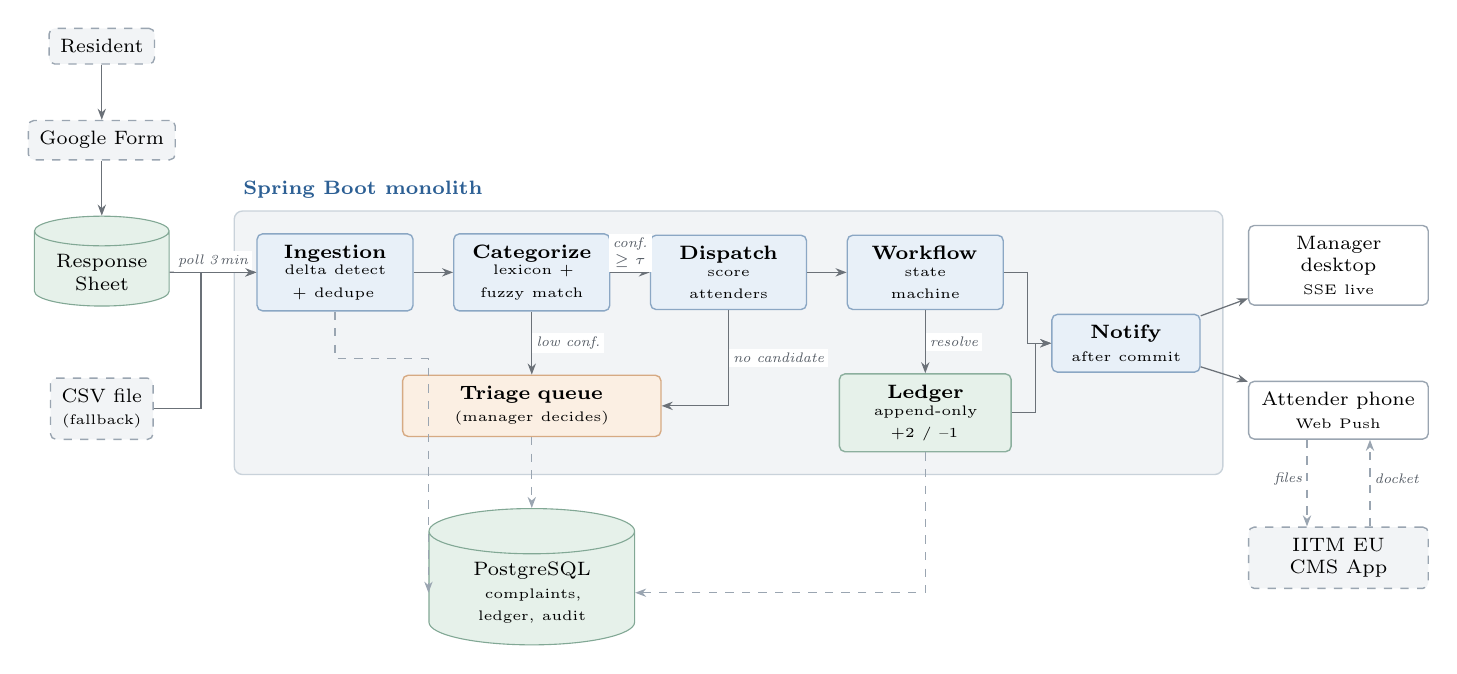
\begin{tikzpicture}[node distance=4mm]

% --- external left ---
\node[ext] (res) {Resident};
\node[ext,below=7mm of res] (gform) {Google Form};
\node[db,below=7mm of gform,text width=15mm] (gsheet) {Response\\Sheet};
\node[ext,below=9mm of gsheet] (csv) {CSV file\\\tiny(fallback)};

\draw[fl] (res) -- (gform);
\draw[fl] (gform) -- (gsheet);

% --- pipeline stages ---
\node[abox,right=11mm of gsheet,text width=17mm] (ing) {\textbf{Ingestion}\\\tiny delta detect\\\tiny + dedupe};
\node[abox,right=5mm of ing,text width=17mm] (cat) {\textbf{Categorize}\\\tiny lexicon +\\\tiny fuzzy match};
\node[abox,right=5mm of cat,text width=17mm] (dis) {\textbf{Dispatch}\\\tiny score\\\tiny attenders};
\node[abox,right=5mm of dis,text width=17mm] (wf) {\textbf{Workflow}\\\tiny state\\\tiny machine};

\draw[fl] (gsheet) -- node[lbl,above]{poll 3\,min} (ing);
\draw[fl] (csv.east) -- ++(6mm,0) |- (ing.west);
\draw[fl] (ing) -- (cat);
\draw[fl] (cat) -- node[lbl,above,align=center]{conf.\\$\ge\tau$} (dis);
\draw[fl] (dis) -- (wf);

% triage drop-out
\node[wbox,below=8mm of cat,text width=30mm] (tri) {\textbf{Triage queue} \tiny(manager decides)};
\draw[fl] (cat.south) -- node[lbl,right]{low conf.} (tri.north);
\draw[fl] (dis.south) |- node[lbl,pos=0.25,right]{no candidate} (tri.east);

% --- ledger + audit ---
\node[gbox,below=8mm of wf,text width=19mm] (led) {\textbf{Ledger}\\\tiny append-only\\\tiny +2 / --1};
\draw[fl] (wf) -- node[lbl,right]{resolve} (led);

% --- storage ---
\node[db,below=9mm of tri,text width=24mm] (pg) {PostgreSQL\\\tiny complaints, ledger, audit};
\draw[fld] (tri) -- (pg);
\draw[fld] (led.south) |- (pg.east);
\draw[fld] (ing.south) -- ++(0,-6mm) -| (pg.west);

% --- notification fan-out ---
\node[abox,right=6mm of wf,text width=16mm,yshift=-9mm] (notif) {\textbf{Notify}\\\tiny after commit};
\draw[fl] (wf.east) -- ++(3mm,0) |- (notif.west);
\draw[fl] (led.east) -- ++(3mm,0) |- (notif.west);

\node[box,above right=1mm and 6mm of notif,text width=20mm] (mgr) {Manager desktop\\\tiny SSE live};
\node[box,below right=1mm and 6mm of notif,text width=20mm] (att) {Attender phone\\\tiny Web Push};
\draw[fl] (notif) -- (mgr);
\draw[fl] (notif) -- (att);

\node[ext,below=11mm of att,text width=20mm] (cms) {IITM EU\\CMS App};
\draw[fld] ([xshift=-4mm]att.south) -- node[lbl,left,pos=0.45]{files} ([xshift=-4mm]cms.north);
\draw[fld] ([xshift=4mm]cms.north) -- node[lbl,right,pos=0.55]{docket} ([xshift=4mm]att.south);

\begin{scope}[on background layer]
  \node[grp,fit=(ing)(wf)(led)(notif)(tri),inner sep=8pt,
        label={[font=\scriptsize\bfseries\color{accent},anchor=south west,yshift=1pt]north west:Spring Boot monolith}] {};
\end{scope}
\end{tikzpicture}
\caption{Context and processing pipeline. Dashed edges are external or persistence links; the
IITM EU CMS app has \emph{no} programmatic integration --- the attender files there manually and
types the returned docket number back into our system.}
\end{figure}

\subsection{Module breakdown}

Root package \code{in.ac.iitm.hostel.duty}. Each module owns exactly one invariant, which is what
makes the boundary meaningful rather than cosmetic.

\begin{tabularx}{\linewidth}{@{}p{2.1cm} p{2.5cm} X@{}}
\toprule
\textbf{Module} & \textbf{Java package} & \textbf{Purpose \& the invariant it owns}\\
\midrule
ingestion & \ttiny{...ingestion} & Fetch rows, detect deltas, normalize into complaints.
  \textit{A source row never becomes two complaints.} \\
categorization & \ttiny{...categorization} & Assign domain + confidence to complaint text.
  \textit{Low confidence never silently becomes a wrong domain.} \\
dispatch & \ttiny{...dispatch} & Score attenders, produce assignments.
  \textit{Every complaint gets an assignment or a recorded triage reason.} \\
workflow & \ttiny{...workflow} & State machine, guards, transitions.
  \textit{Only legal transitions occur, atomically with their side effects.} \\
ledger & \ttiny{...ledger} & Point movements, leaderboard projection.
  \textit{Append-only; no double-credit; balance is derived, never stored.} \\
notification & \ttiny{...notification} & Outbox fan-out to manager SSE and attender Web Push.
  \textit{Best-effort; never blocks a transaction.} \\
analytics & \ttiny{...analytics} & MTTR, bottlenecks, anomaly detection.
  \textit{Read-only over ledger and audit.} \\
reporting & \ttiny{...reporting} & \code{.xlsx} generation via Apache POI.
  \textit{Reports are reproducible point-in-time snapshots.} \\
identity & \ttiny{...identity} & Users, roles, Google allowlist, manager password, provisioning.
  \textit{No self-registration; every principal is pre-provisioned.} \\
audit & \ttiny{...audit} & Append-only event log.
  \textit{Written in the same transaction as the change it records.} \\
\bottomrule
\end{tabularx}

\subsection{Layering}

\code{web} $\rightarrow$ \code{application} $\rightarrow$ \code{domain}, with
\code{infrastructure} implementing domain-facing ports. Four rules, enforced by ArchUnit in CI:

\begin{enumerate}
  \item \code{domain} depends on nothing but the JDK --- no Spring, no JPA behaviour.
  \item \code{web} never touches a repository; it goes through \code{application}.
  \item Cross-module calls use the target's published service interface, never its internals.
  \item \code{@Transactional} lives only in \code{application}.
\end{enumerate}

Rule 4 matters more than it looks: transaction boundaries are where the concurrency guarantees are
enforced, so they must sit in one predictable place.

\subsection{Deployment topology}

\begin{figure}[H]
\centering
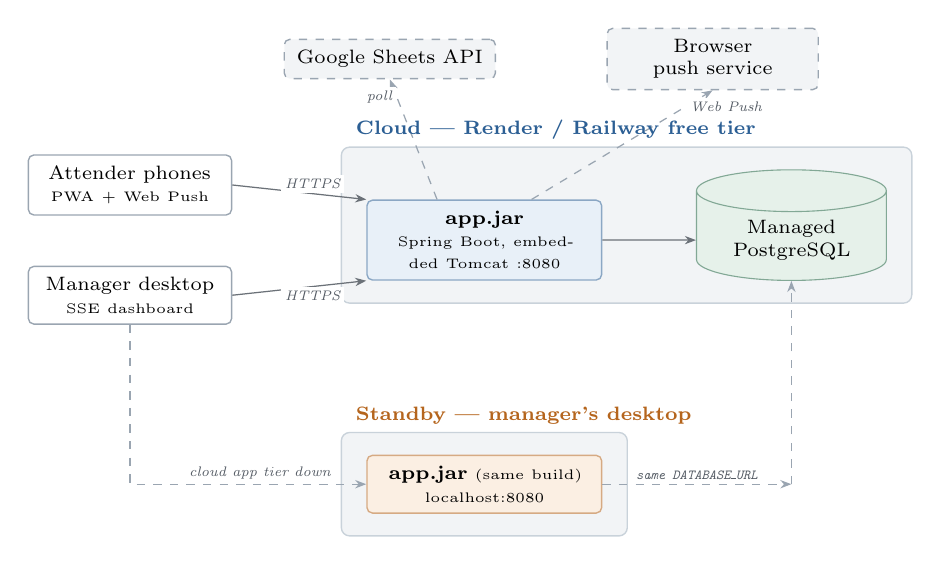
\begin{tikzpicture}[x=1cm,y=1cm]

% ---- external services, kept clear of the group boxes ----
\node[ext,text width=24mm] (gs)  at (1.9, 2.85) {Google Sheets API};
\node[ext,text width=24mm] (wp)  at (6.0, 2.85) {Browser push service};

% ---- cloud ----
\node[abox,text width=27mm] (jar) at (3.1, 0.55) {\textbf{app.jar}\\\tiny Spring Boot, embedded Tomcat :8080};
\node[db,text width=22mm]   (pgc) at (7.0, 0.55) {Managed\\PostgreSQL};
\draw[fl] (jar) -- (pgc);

% ---- clients ----
\node[box,text width=23mm] (phone) at (-1.4, 1.25) {Attender phones\\\tiny PWA + Web Push};
\node[box,text width=23mm] (desk)  at (-1.4,-0.15) {Manager desktop\\\tiny SSE dashboard};
\draw[fl] (phone.east) -- node[lbl,above,pos=0.6]{HTTPS} (jar.north west);
\draw[fl] (desk.east)  -- node[lbl,below,pos=0.6]{HTTPS} (jar.south west);

% ---- standby ----
\node[wbox,text width=27mm] (jarl) at (3.1,-2.55) {\textbf{app.jar} \tiny(same build)\\\tiny localhost:8080};

\draw[fld] (desk.south) -- (-1.4,-2.55) -- node[lbl,above,pos=0.55]{cloud app tier down} (jarl.west);
\coordinate (join) at (7.0,-2.55);
\draw[fld] (jarl.east) -- node[lbl,above]{\ttfamily same DATABASE\_URL} (join);
\draw[fld] (join) -- (pgc.south);
\draw[fld] ([xshift=6mm]jar.north) -- node[lbl,right,pos=0.85]{Web Push} (wp.south);
\draw[fld] ([xshift=-6mm]jar.north) -- node[lbl,left,pos=0.85]{poll} (gs.south);

\begin{scope}[on background layer]
  \node[grp,fit=(jar)(pgc),inner xsep=9pt,inner ysep=8pt] (cb) {};
  \node[grp,fit=(jarl),inner xsep=9pt,inner ysep=8pt] (fb) {};
\end{scope}
\node[font=\scriptsize\bfseries\color{accent},anchor=west] at ([xshift=2pt,yshift=6pt]cb.north west)
  {Cloud --- Render / Railway free tier};
\node[font=\scriptsize\bfseries\color{warm},anchor=west] at ([xshift=2pt,yshift=6pt]fb.north west)
  {Standby --- manager's desktop};
\end{tikzpicture}
\caption{Deployment. \textbf{One database.} The standby is the same jar with the same
\code{DATABASE\_URL}, started on the manager's desktop when the cloud app tier is down. The outage
designed for is the \emph{platform} failing, not the network.}
\end{figure}

\begin{tabularx}{\linewidth}{@{}p{2.6cm} X X@{}}
\toprule
& \textbf{Cloud (primary)} & \textbf{Standby (manager's desktop)}\\
\midrule
Database & Managed PostgreSQL & \textbf{The same} managed PostgreSQL \\
Reached by & Attenders and manager, HTTPS & Manager only, on \code{localhost} \\
Ingestion & Sheets polling + CSV & Both --- internet is available \\
Notifications & SSE + Web Push & SSE + Web Push \\
Authentication & Google (attenders) + password (manager) & Manager password --- no Google round-trip \\
Purpose & Day-to-day operation & Continuity when the app tier is down \\
\bottomrule
\end{tabularx}

Free-tier instances sleep when idle, so \code{@Scheduled} polling alone is unreliable. Mitigations:
a \textbf{Sync~Now} button that is the guaranteed path and also wakes the instance, and catch-up
ingestion on startup --- safe because delta detection is watermark-based rather than time-based, so
a six-hour gap and a six-minute gap take the identical code path.

An earlier draft ran the standby on embedded H2 seeded from a nightly dump. That forced every
migration into the SQL subset both engines accept, and left an unsolved problem: \textbf{work done
during an outage had no path back into the cloud database.} Two diverging copies of the points
ledger is precisely the failure this system exists to prevent --- one database means it cannot
arise. Residual risk is the managed database failing, which no application design fixes.

% =========================== 4. DATA MODEL ==================================
\section{Data Model}

\subsection{Design principles}

\begin{enumerate}
  \item \textbf{Facts are immutable; state is derived.} Point balances are never a mutable counter
        --- they are a \code{SUM} over an append-only ledger. This makes double-crediting a
        constraint violation rather than a race to win.
  \item Every mutable aggregate root carries a \code{version} column for optimistic locking.
  \item Audit rows are written \emph{inside the same transaction} as the change they record, so
        the log can never disagree with the data.
  \item No hard deletes on operational data; rows are tombstoned.
\end{enumerate}

\subsection{Entity--relationship model}

\begin{figure}[H]
\centering
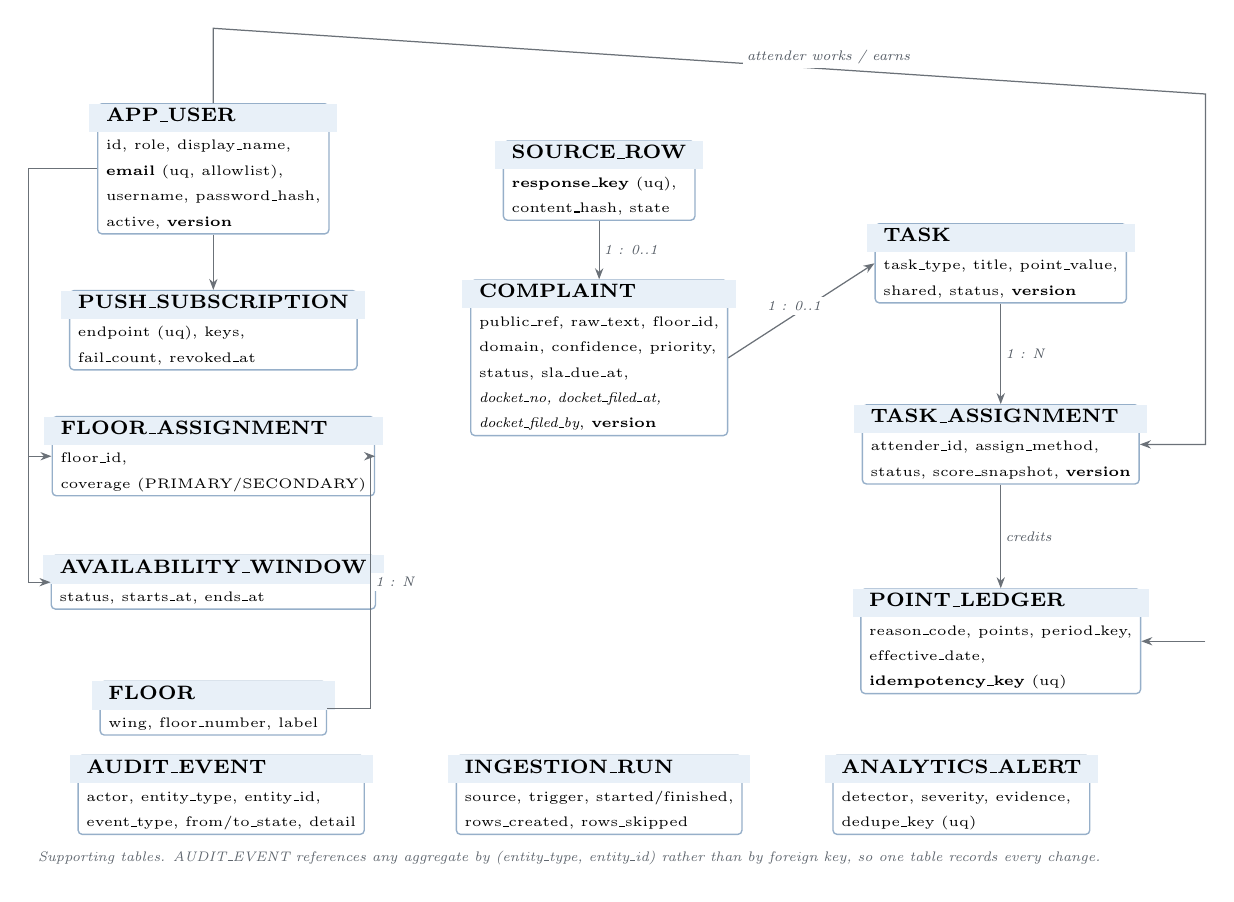
\begin{tikzpicture}[x=1cm,y=1cm,every node/.style={font=\scriptsize}]

\newcommand{\entity}[4]{%
  \node[ent] (#2) at (#1) {%
    \begin{tabular}{@{\hspace{3pt}}l@{\hspace{3pt}}}
      \cellcolor{accentlt}\textbf{#3}\\[1pt] #4
    \end{tabular}};}

% ---- column 1: identity & coverage ----
\entity{0,0}{user}{APP\_USER}{\tiny id, role, display\_name,\\\tiny \textbf{email} (uq, allowlist),\\\tiny username, password\_hash,\\\tiny active, \textbf{version}}
\entity{0,-2.05}{push}{PUSH\_SUBSCRIPTION}{\tiny endpoint (uq), keys,\\\tiny fail\_count, revoked\_at}
\entity{0,-3.65}{floora}{FLOOR\_ASSIGNMENT}{\tiny floor\_id,\\\tiny coverage (PRIMARY/SECONDARY)}
\entity{0,-5.25}{avail}{AVAILABILITY\_WINDOW}{\tiny status, starts\_at, ends\_at}
\entity{0,-6.85}{floorent}{FLOOR}{\tiny wing, floor\_number, label}

% ---- column 2: ingestion & complaint ----
\entity{4.9,-0.15}{src}{SOURCE\_ROW}{\tiny \textbf{response\_key} (uq),\\\tiny content\_hash, state}
\entity{4.9,-2.4}{comp}{COMPLAINT}{\tiny public\_ref, raw\_text, floor\_id,\\\tiny domain, confidence, priority,\\\tiny status, sla\_due\_at,\\\tiny \textit{docket\_no, docket\_filed\_at,}\\\tiny \textit{docket\_filed\_by}, \textbf{version}}

% ---- column 3: work & points ----
\entity{10.0,-1.2}{task}{TASK}{\tiny task\_type, title, point\_value,\\\tiny shared, status, \textbf{version}}
\entity{10.0,-3.5}{asg}{TASK\_ASSIGNMENT}{\tiny attender\_id, assign\_method,\\\tiny status, score\_snapshot, \textbf{version}}
\entity{10.0,-6.0}{ledger}{POINT\_LEDGER}{\tiny reason\_code, points, period\_key,\\\tiny effective\_date,\\\tiny \textbf{idempotency\_key} (uq)}

% ---- relations: APP_USER owns the left column (vertical bus) ----
\draw[fl] (user.south) -- (push.north);
\coordinate (bus) at (-2.35,0);
\draw[draw=ink!65,line width=0.45pt] (user.west) -- (bus);
\draw[draw=ink!65,line width=0.45pt] (bus) -- (-2.35,-5.25);
\foreach \n in {floora,avail}{\draw[fl] (\n.west -| bus) -- (\n.west);}
\draw[fl] (floorent.east) -- ++(0.55,0) |- node[lbl,right,pos=0.25]{1 : N} (floora.east);

% ---- ingestion chain ----
\draw[fl] (src.south) -- node[lbl,right]{1 : 0..1} (comp.north);

% ---- complaint -> work ----
\draw[fl] (comp.east) -- node[lbl,above,pos=0.45]{1 : 0..1} (task.west);
\draw[fl] (task.south) -- node[lbl,right]{1 : N} (asg.north);
\draw[fl] (asg.south)  -- node[lbl,right]{credits} (ledger.north);

% ---- attender -> work (routed over the top) ----
\draw[fl] (user.north) -- ++(0,0.95) -- node[lbl,above,pos=0.62]{attender works / earns} (12.6,0.95)
          -- (12.6,-3.5) -- (asg.east);
\draw[fl] (12.6,-6.0) -- (ledger.east);

% ---- cross-cutting tables ----
\entity{0.1,-7.95}{audit}{AUDIT\_EVENT}{\tiny actor, entity\_type, entity\_id,\\\tiny event\_type, from/to\_state, detail}
\entity{4.9,-7.95}{run}{INGESTION\_RUN}{\tiny source, trigger, started/finished,\\\tiny rows\_created, rows\_skipped}
\entity{9.5,-7.95}{alert}{ANALYTICS\_ALERT}{\tiny detector, severity, evidence,\\\tiny dedupe\_key (uq)}
\node[font=\tiny\itshape,text=ink!70,anchor=west] at (-2.35,-8.75)
  {Supporting tables. AUDIT\_EVENT references any aggregate by (entity\_type, entity\_id) rather than by foreign key, so one table records every change.};
\end{tikzpicture}
\caption{Core entities. Bold fields carry the guarantees: \code{version} for optimistic locking,
\code{response\_key} for ingestion identity, \code{idempotency\_key} for point integrity.}
\end{figure}

\subsection{The two constraints that carry the design}

\begin{tabularx}{\linewidth}{@{}p{4.5cm} X@{}}
\toprule
\textbf{Constraint} & \textbf{What it prevents}\\
\midrule
\ttiny{uq\_source\_row}\newline\tiny(source, \textbf{response\_key}) &
  A source row becoming two complaints. Identity is
  \code{SHA256(timestamp\,$\|$\,email)} --- \emph{not} row index, because deleting one sheet row
  shifts every index below it and a positional key would report the whole tail as amended. \\
\ttiny{uq\_ledger\_idem}\newline\tiny(\textbf{idempotency\_key}) &
  Double-crediting. The key is derived from the \emph{work}
  (\code{RESOLVE:\{task\}:\{attender\}}), not the request, so a retry on flaky hostel Wi-Fi ---
  the expected case, not an exotic one --- collides and is swallowed as a no-op. \\
\bottomrule
\end{tabularx}

\keybox{Consequence.}{There is no \code{attender.points} column anywhere in the schema. No counter
to increment means no lost update on a counter, and nothing to reconcile. A balance is a \code{SUM}
over immutable facts, which is also what lets a bonus dispute be answered line by line.}

\subsection{Audit log}

Every state change, point movement, authentication attempt and configuration change is written to
\code{audit\_event}. It is the evidence base for bonus disputes, so it is designed to be
trustworthy rather than decorative.

\begin{tabularx}{\linewidth}{@{}p{2.9cm} X@{}}
\toprule
\textbf{Column} & \textbf{Content}\\
\midrule
\ttiny{occurred\_at} & UTC instant of the change \\
\ttiny{actor\_id, actor\_role} & Who did it. \code{NULL} for system/scheduler actions \\
\ttiny{on\_behalf\_of} & Set when the manager used \code{act-as}; the points still go to the attender \\
\ttiny{entity\_type, entity\_id} & What was changed --- \code{COMPLAINT}, \code{TASK}, \code{LEDGER}, \code{APP\_USER}, \dots \\
\ttiny{event\_type} & \code{TRANSITION}, \code{POINTS\_CREDITED}, \code{PENALTY\_LOGGED}, \code{SIGN\_IN}, \code{SIGN\_IN\_REJECTED}, \code{USER\_PROVISIONED}, \code{CONFIG\_CHANGED}, \dots \\
\ttiny{from\_state, to\_state} & For transitions, the exact edge taken \\
\ttiny{detail} & JSON payload: reason text, dispatch score snapshot, old/new config values \\
\ttiny{correlation\_id} & Groups everything caused by one request or one ingestion run \\
\bottomrule
\end{tabularx}

Two properties make it dependable. It is written by a \code{BEFORE\_COMMIT} transactional event
listener, so it \textbf{commits atomically} with the change it records and can never silently
diverge. And there is \textbf{no code path that updates or deletes an audit row} --- the JPA entity
exposes no setters and the repository no delete method. Combined with the append-only ledger, an
attender's monthly bonus can be reconstructed from first principles and defended line by line.

% =========================== 5. STATE MACHINE ===============================
\section{Complaint \& Task Lifecycle}

Status is the most-read field in the system: it drives the attender queue, the dashboard, SLA
aging, MTTR measurement and the point credit. Leaving it as an informally-updated string is how a
ticket ends up \code{RESOLVED} with no docket, or credited twice.

The \emph{only} way to change it is
\code{WorkflowService.transition(id, event, actor, payload)}, which loads the aggregate with its
\code{version}, rejects any \code{(state, event)} pair absent from the transition table, evaluates
the guard, then applies the change, its side effects and the audit row \textbf{in one transaction};
notifications fire separately on \code{AFTER\_COMMIT}. Controllers, the scheduler and the CSV importer all funnel through it.

\begin{figure}[H]
\centering
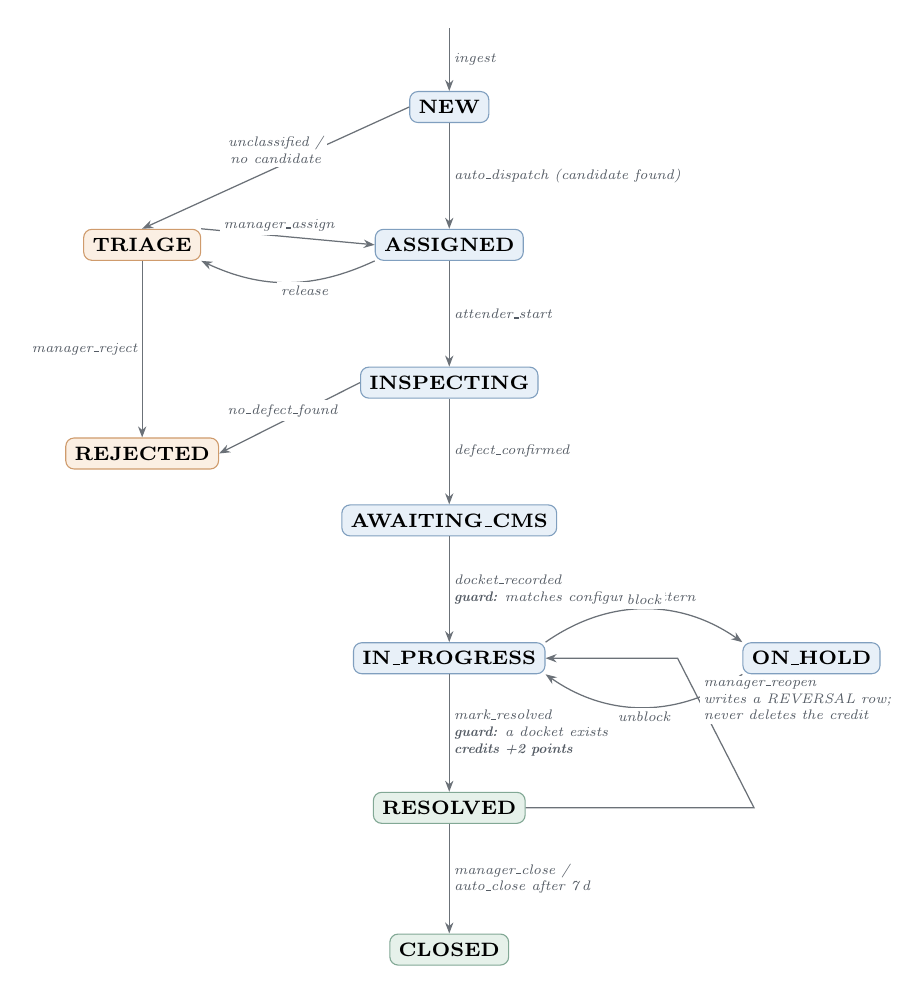
\begin{tikzpicture}[x=1cm,y=1cm]

% ---- happy path, vertical ----
\node[st] (new)   at (4.6, 0)    {NEW};
\node[st] (asg)   at (4.6,-1.75) {ASSIGNED};
\node[st] (insp)  at (4.6,-3.5)  {INSPECTING};
\node[st] (await) at (4.6,-5.25) {AWAITING\_CMS};
\node[st] (prog)  at (4.6,-7.0)  {IN\_PROGRESS};
\node[stend] (res) at (4.6,-8.9) {RESOLVED};
\node[stend] (clo) at (4.6,-10.7){CLOSED};

% ---- branches ----
\node[st,draw=warm!65,fill=warmlt] (tri) at (0.7,-1.75) {TRIAGE};
\node[strej] (rej) at (0.7,-4.4) {REJECTED};
\node[st] (hold)   at (9.2,-7.0) {ON\_HOLD};

\coordinate (start) at (4.6,1.0);
\draw[fl] (start) -- node[lbl,right]{ingest} (new);

% main chain
\draw[fl] (new)  -- node[lbl,right,align=left]{auto\_dispatch \tiny(candidate found)} (asg);
\draw[fl] (asg)  -- node[lbl,right]{attender\_start} (insp);
\draw[fl] (insp) -- node[lbl,right]{defect\_confirmed} (await);
\draw[fl] (await)-- node[lbl,right,align=left]{docket\_recorded\\\tiny \textbf{guard:} matches configured pattern} (prog);
\draw[fl] (prog) -- node[lbl,right,align=left]{mark\_resolved\\\tiny \textbf{guard:} a docket exists\\\tiny \textbf{credits +2 points}} (res);
\draw[fl] (res)  -- node[lbl,right,align=left]{manager\_close /\\auto\_close after 7\,d} (clo);

% triage branch
\draw[fl] (new.west)  -- node[lbl,above,align=center,pos=0.5]{unclassified /\\no candidate} (tri.north);
\draw[fl] (tri.north east) -- node[lbl,above,pos=0.45,align=center]{manager\_assign} (asg.west);
\draw[fl] (asg.south west) to[out=205,in=-25] node[lbl,below,pos=0.4]{release} (tri.south east);
\draw[fl] (tri) -- node[lbl,left]{manager\_reject} (rej);
\draw[fl] (insp.west) -- node[lbl,above,pos=0.55]{no\_defect\_found} (rej.east);

% hold
\draw[fl] (prog.north east) to[out=35,in=145] node[lbl,above]{block} (hold.north west);
\draw[fl] (hold.south west) to[out=215,in=-35] node[lbl,below]{unblock} (prog.south east);

% reopen
\draw[fl] (res.east) -- ++(2.9,0) -- node[lbl,right,align=left,pos=0.72]{manager\_reopen\\\tiny writes a REVERSAL row;\\\tiny never deletes the credit} (7.5,-7.0) -- (prog.east);
\end{tikzpicture}
\caption{Complaint lifecycle. Two guards carry the institutional requirements: a docket must match
the configured pattern to be recorded, and \textbf{a complaint cannot be resolved for points
without one}.}
\end{figure}

\subsection{Two guards worth calling out}

\textbf{The docket gate.} \code{mark\_resolved} requires a docket to exist. This makes
institutional traceability structurally enforced rather than a matter of attender diligence ---
you cannot collect +2 points for a complaint you never filed with the Engineering Unit. Because
there is no CMS API, we validate \emph{format} only, and the pattern is configuration, so a wrong
guess costs a property change rather than a redeploy.

\textbf{Reopen reverses, never deletes.} The ledger is append-only, so a reopen writes a
compensating \code{REVERSAL} row; both the original credit and the reversal stay visible.
Re-resolving afterwards writes a new credit under key
\code{RESOLVE:\{task\}:\{attender\}:r\{n\}}, so the idempotency guarantee survives the reopen cycle
without ever blocking legitimate repeat work.

\subsection{Special duties}

Special duties have no complaint and no docket:
\code{OPEN} $\rightarrow$ \code{CLAIMED} $\rightarrow$ \code{COMPLETED}, with
\code{CANCELLED} and \code{EXPIRED} exits. For a \textbf{shared} duty several attenders hold active
assignments at once; the duty completes when every assignee has marked their part done, and
\emph{each} is credited once under their own key \code{DUTY:\{task\}:\{attender\}}.

\subsection{Priority logic}

Priority is not a fixed label --- it ages, so old low-priority work eventually surfaces above new
noise.

\begin{tabularx}{\linewidth}{@{}l X l@{}}
\toprule
\textbf{Base} & \textbf{Assigned when} & \textbf{Initial SLA}\\
\midrule
\code{P1} & Safety keywords matched \textbf{exactly} --- \textit{shock, spark, short circuit,
  sewage, no water, overflow}. No fuzzy matching here: a false P1 from a near-miss spelling would
  distort the whole queue. & Electrical 4\,h\newline Other 8\,h \\
\code{P2} & Default for a confidently classified complaint & Elec 8\,h, RO 12\,h,\newline Civil /
  Network 24\,h \\
\code{P3} & Cosmetic keywords, or downgraded by the manager & 72\,h \\
\bottomrule
\end{tabularx}

A scheduled job escalates \code{P3}\,$\rightarrow$\,\code{P2}\,$\rightarrow$\,\code{P1} once a
complaint has been open past \textbf{1.5$\times$} its SLA window without reaching \code{RESOLVED}.
\code{base\_priority} is retained, so the dashboard can always show ``P1 (aged from P3)''.
Escalation caps at \code{P1}, and \textbf{hold time does not count toward it} --- otherwise
``waiting three days for the Engineering Unit to send a plumber'' would be recorded as attender
slowness and would point the bottleneck analysis at exactly the wrong place.

% =========================== 6. DISPATCH ====================================
\section{Dispatch Heuristic}

Given a classified complaint $c$ and attenders $A$, choose who should do the work. The formulation
must always terminate with an assignment \emph{or} a recorded triage reason, be deterministic
including tie-breaks, be explainable to the manager, avoid starvation, and be tunable without a
redeploy.

\subsection{Stage 1 --- hard eligibility filter}

\[ E=\{\,a\in A \;:\; a.\mathrm{active}\ \wedge\ \mathrm{availability}(a,\mathrm{now})=\texttt{AVAILABLE}\ \wedge\ \neg\,\mathrm{assigned}(a,c)\,\} \]

Availability is a \textbf{gate, not a score}. Someone on leave must never be chosen no matter how
well they score elsewhere; folding it into a weighted sum would let a strong floor match outvote
the fact that a person is not at work. If $E=\varnothing$ the complaint goes to \code{TRIAGE} with
reason \code{NO\_AVAILABLE\_ATTENDER} --- the proposal's ``all floor attenders unavailable'' edge
case, handled by construction rather than a special branch.

\subsection{Stage 2 --- score the eligible set}

\[ \mathrm{Score}(a,c)=w_f\!\cdot\!\mathrm{Floor}(a,c)\;+\;w_l\!\cdot\!\mathrm{Load}(a) \]

Two terms, each normalised to $[0,1]$, weights summing to 1, so $\mathrm{Score}\in[0,1]$ and each
weight reads directly as ``how much does this factor matter''.

\begin{tabularx}{\linewidth}{@{}p{2.45cm} p{1.15cm} X@{}}
\toprule
\textbf{Term} & \textbf{Weight} & \textbf{Definition}\\
\midrule
\textbf{Floor} proximity & $w_f=0.60$ &
  \code{PRIMARY} coverage $=1.00$; \code{SECONDARY} $=0.70$; adjacent floor same wing $=0.40$;
  same wing $|\Delta|\!\ge\!2$ is $\max(0.10,\,0.35-0.05|\Delta|)$; different wing $=0.10$.
  Non-zero for distant attenders on purpose: when the primary is away someone still has to go. \\
\textbf{Load} (free capacity) & $w_l=0.40$ &
  $L(a)=\sum_t \pi(t)$ over active tasks with $\pi(\text{P1})\!=\!3,\pi(\text{P2})\!=\!2,\pi(\text{P3})\!=\!1$;
  $\mathrm{Load}(a)=1-\min(1,L(a)/L_{cap})$, $L_{cap}=8$. Weighting by priority reflects reality ---
  three P1 electrical faults is not three P3 cosmetic complaints. \code{ON\_HOLD} counts 0. \\
\bottomrule
\end{tabularx}

\textbf{Two terms were cut, and the reason generalises.} An earlier draft added a \emph{domain
skill} term and a \emph{continuity} term. Skill defaulted to a neutral $0.5$ for every attender,
because we do not know whether attenders specialise --- and a constant added identically to every
candidate \textbf{cannot change the ranking}. It was arithmetic that looked like intelligence.
Continuity (has this attender worked this room lately?) carried 10\% weight and cost a 14-day
lookback query per candidate; the signal it captures is used to better effect by the chronic-defect
detector, which tells the manager to \emph{replace the fixture} rather than merely routing the next
complaint to the same person. What remains is a dozen lines of pure Java with no framework
involvement.

\subsection{Stage 3 --- select, tie-break, record}

$\mathrm{best}=\arg\max_{a\in E}\mathrm{Score}(a,c)$, with ties broken in strict order:
(1)~fewest tasks assigned \emph{today} --- the anti-starvation term; (2)~longest time since last
assignment; (3)~lowest user id, which guarantees full determinism.

The complete score breakdown is persisted to \code{task\_assignment.score\_snapshot} as JSON
(chosen attender, each component, the weights, runners-up, tie-break used). This is what makes
``why did Ravi get this?'' answerable months later, and it is what the dashboard renders in the
assignment tooltip.

\subsection{Degenerate cases}

\begin{tabularx}{\linewidth}{@{}p{5.0cm} X@{}}
\toprule
\textbf{Case} & \textbf{Outcome}\\
\midrule
No attender available ($E=\varnothing$) & \code{TRIAGE} / \code{NO\_AVAILABLE\_ATTENDER} \\
Room number unparseable & \code{TRIAGE} / \code{UNMAPPED\_LOCATION} --- dispatching on a location we could not read is worse than asking \\
Floor exists, nobody covers it & Assign least-loaded, warn \code{UNCOVERED\_FLOOR} \\
Every attender at capacity & Assign best anyway, notify \code{CapacityExceeded}. Overflowing visibly beats triaging silently \\
Complaint \code{UNCLASSIFIED} & Never reaches dispatch; triaged at classification \\
Manager disagrees & \code{manager\_reassign}; both assignments audited \\
\bottomrule
\end{tabularx}

\keybox{Why greedy, not optimal assignment?}{A global optimum (Hungarian, min-cost flow) is
rejected deliberately. Complaints arrive \emph{one at a time} from a 3-minute poll, so a typical
batch is 1--3 items --- and the optimal assignment of a one-item batch \emph{is} the greedy one.
With $|A|=4$ the theoretical gain is negligible, while batch optimisation would mean holding
complaints back to accumulate a batch, adding latency to exactly the P1 cases that matter most.
Greedy is also arguable: ``Ravi 0.78 vs Kumar 0.50'' is something a manager can push back on.}

% =========================== 7. PII =========================================
\section{PII \& Data Protection}

Complaints originate from residents, so the system holds personal data about people who never
agreed to use it and cannot log in to check what we keep. That asymmetry drives a minimisation-first
stance.

\begin{tabularx}{\linewidth}{@{}p{3.4cm} X p{2.9cm}@{}}
\toprule
\textbf{Data} & \textbf{Why held} & \textbf{Retention}\\
\midrule
Resident email & Contacting the reporter when details are unclear & 90 days, then nulled \\
Room number & \textbf{Operationally essential} --- dispatch depends on it & 1 year \\
Complaint text & Diagnosis, classification, chronic-defect detection & 1 year, then \code{[purged]} \\
Attender name & Assignment, leaderboard & Life of employment \\
Attender Google email & Allowlist key; identifies the actor in the audit log & Life of employment \\
Push endpoint + keys & Delivering assignment alerts & Until revoked or 3 failures \\
Audit log, point ledger & Bonus dispute resolution & Indefinite \\
\bottomrule
\end{tabularx}

\textbf{What we deliberately do not collect.} Resident names and phone numbers are simply omitted
from the ingestion column map, even when the Google Form offers them. The cheapest way to protect
personal data is not to hold it.

\textbf{Aggregates survive purging.} MTTR, arrival counts and chronic-defect detection all depend
on timestamps, domain and room --- not on what the resident wrote --- so analytics keeps working
after text redaction. Similarly, \code{source\_row.raw\_payload} is purged at 90 days while
\code{content\_hash} is retained, so we can still recognise a previously-seen row without storing
what it said: retention and idempotency coexist rather than trade off.

\textbf{Push payloads} are end-to-end encrypted (\code{aes128gcm}), so Google's or Mozilla's relay
sees only ciphertext. Notification bodies still name \emph{a room, never a person} --- a lock-screen
preview is visible to anyone holding the phone.

\textbf{Test fixtures are anonymised at extraction}, before real data ever enters the repository.
A committed fixture is effectively permanent, so the scrub cannot be a later step: emails become
\code{resident\{n\}@example.com}, names are removed, and room numbers are remapped through a fixed
permutation that preserves floor structure (keeping dispatch tests meaningful) while breaking
identifiability. The mapping table is not committed.

\textbf{Secrets} live only in environment variables --- the Google service-account key (base64),
\code{DATABASE\_URL}, \code{APP\_SECRET}, and the VAPID key pair. \code{.gitignore} blocks the
obvious filenames and CI runs Gitleaks on every pull request, so a committed credential fails the
build rather than reaching \code{main}. The Sheets service account is granted \textbf{read-only}
access to a single sheet.

% =========================== 8. TECH STACK ==================================
\section{Technology Stack by Module}

\textbf{Language} Java 21 \quad\textbullet\quad \textbf{Build} Maven \quad\textbullet\quad
\textbf{Framework} Spring Boot 3.x \quad\textbullet\quad \textbf{Database} PostgreSQL 16
\quad\textbullet\quad \textbf{Packaging} single executable \code{.jar}

\begin{tabularx}{\linewidth}{@{}p{2.35cm} X p{3.05cm}@{}}
\toprule
\textbf{Module} & \textbf{Libraries \& technology} & \textbf{Milestone}\\
\midrule
identity &
  Spring Security 6: OAuth2 client (Google OIDC) for attenders, form login + BCrypt cost 12
  for the manager, custom \code{OidcUserService} for the allowlist &
  S1 \textit{(12--18 Sep)} \\
persistence &
  Spring Data JPA / Hibernate 6, Flyway (forward-only migrations), HikariCP,
  Testcontainers for tests &
  S1 \\
ingestion &
  \code{google-api-services-sheets:v4} + service-account auth; Apache Commons CSV for the
  fallback adapter; SHA-256 via JDK \code{MessageDigest} &
  S2 \textit{(19--25 Sep)} \\
categorization &
  Hand-built weighted lexicon; Apache Commons Text (Levenshtein, Jaro--Winkler) for fuzzy
  matching. \textit{Apache OpenNLP \code{DocumentCategorizer} deferred to an optional second
  stage} &
  S2 \\
dispatch &
  Plain Java domain code, no framework. Weights bound via
  \code{@ConfigurationProperties} &
  S3 \textit{(26 Sep--2 Oct)} \\
workflow &
  Hand-rolled transition table over a Java \code{enum}. \textit{Spring Statemachine was
  considered and rejected --- our guards need transactional side effects, which is simpler to
  express directly} &
  S3 \\
ledger &
  JPA with \code{@Version}; correctness carried by a database \code{UNIQUE} constraint rather
  than application logic &
  S3 \\
scheduling &
  Spring \code{@Scheduled} / \code{@Async}; ShedLock for distributed lock safety &
  S2--S3 \\
web (manager) &
  Thymeleaf, Tailwind CSS (purged), Chart.js 4 &
  S4 \textit{(3--9 Oct)} \\
web (attender) &
  Thymeleaf server-rendered shell + PWA service worker (push receiver) &
  S4 \\
validation &
  Hibernate Validator (Jakarta Bean Validation) --- entity constraints, CMS docket pattern &
  S3--S4 \\
deployment &
  Docker Compose locally; \code{.jar} on Render / Railway with managed PostgreSQL &
  S4 \\
concurrency &
  JPA optimistic locking; \code{SELECT \dots FOR UPDATE} for duty claims only &
  S5 \textit{(10--16 Oct)} \\
analytics &
  Plain Java statistics (median, MAD, EWMA, Poisson tail) over JPQL aggregates.
  \textit{No stats library --- the five estimators we need are a few lines each and stay
  explainable} &
  S6 \textit{(17--23 Oct)} \\
reporting &
  Apache POI (\code{poi-ooxml}) for multi-tab \code{.xlsx} export &
  S7 \textit{(24--30 Oct)} \\
notification &
  Spring MVC \code{SseEmitter} on \code{AFTER\_COMMIT}; \code{nl.martijndwars:web-push}
  with VAPID for attender push &
  S7 \\
testing &
  JUnit 5, AssertJ, Mockito, Testcontainers, ArchUnit, JaCoCo &
  Throughout \\
CI/CD &
  GitHub Actions (\code{mvn verify}), Gitleaks, OWASP Dependency-Check, Dependabot &
  S1 \\
\bottomrule
\end{tabularx}

% =========================== 9. TEST PLAN ===================================
\section{Test Plan}

\begin{tabularx}{\linewidth}{@{}p{2.3cm} p{3.6cm} X p{1.1cm}@{}}
\toprule
\textbf{Level} & \textbf{Tooling} & \textbf{Scope} & \textbf{Share}\\
\midrule
Unit & JUnit 5, AssertJ & Pure domain logic --- scoring, classification, transitions, statistics. No Spring context & 70\% \\
Slice & \code{@DataJpaTest}, \code{@WebMvcTest} & Repositories against real Postgres; controller contracts & 15\% \\
Integration & \code{@SpringBootTest} + Testcontainers & Full pipeline, transactions, concurrency & 10\% \\
Concurrency & \code{CountDownLatch}, \code{ExecutorService} & The five named races & named suite \\
Architecture & ArchUnit & Layering rules of Sec.~3.4 & continuous \\
Acceptance & Stakeholder walkthrough & The manager's own criteria & per milestone \\
\bottomrule
\end{tabularx}

\textbf{All database tests run against real PostgreSQL via Testcontainers}, never an in-memory
substitute. The properties we most need to verify --- unique-constraint behaviour under concurrent
inserts, optimistic-lock failures, row locking --- are precisely the ones an H2 stand-in would fake
convincingly and wrongly. Coverage floor: 75\% line, 90\% on \code{domain}, gated in CI.

\subsection{Fixtures}

\begin{tabularx}{\linewidth}{@{}p{1.1cm} p{4.6cm} X@{}}
\toprule
& \textbf{Fixture} & \textbf{Purpose}\\
\midrule
F1 & $\sim$200 real complaints, anonymised & Classifier gold set; realistic dispatch \\
F2 & $\sim$60 hand-authored edge cases & Corner-case suite \\
F3 & 4 attenders $\times$ 25 tasks & Concurrency races \\
F4 & 90 days, $\sim$1800 complaints & Analytics and anomaly detectors \\
F5 & $\sim$30 malformed sheet rows & Ingestion robustness \\
\bottomrule
\end{tabularx}

\subsection{Proving the 90\% categorization criterion}

The acceptance criterion needs a definition that cannot be gamed, so we fix one now. F1 is labelled
by hand and split \textbf{70/30 into development and holdout}; the lexicon and thresholds are tuned
\emph{only} against development, and the holdout is scored once per milestone --- tuning against it
would produce a number that means nothing.

\[ \text{coverage}=\frac{\text{auto-accepted}}{\text{total}} \qquad
   \text{accuracy}=\frac{\text{correct}}{\text{auto-accepted}} \]

\textbf{Both are always reported together}, because accuracy alone is trivially gameable: a
classifier that refuses to classify anything scores 100\%. Targets: \textbf{accuracy $\ge$ 90\%,
coverage $\ge$ 70\%}, with a per-domain confusion matrix. Items a human labelled \code{AMBIGUOUS}
are expected to reach triage; auto-accepting one counts as an error. In production every manager
triage correction is a free \code{(text, true label)} pair, giving a growing corpus for monthly
drift re-scoring.

\subsection{Corner cases (selected from 31)}

\begin{tabularx}{\linewidth}{@{}p{6.3cm} X@{}}
\toprule
\textbf{Case} & \textbf{Expected}\\
\midrule
Identical simultaneous submissions, two residents & Two complaints --- distinct \code{response\_key} \\
Byte-identical resubmission by one resident & One complaint --- key collides \\
Same CSV uploaded twice by mistake & Zero duplicates \\
Sheet row deleted, shifting all indices below & \textbf{Zero spurious amendments} \\
Sheet row deleted entirely & Ignored --- the sheet is an inbox, the complaint is unaffected \\
Required column renamed & Run fails loudly, never a silent partial ingest \\
Tamil-transliterated text (``thanni varala'') & Lexicon/fuzzy hit or triage --- never a confident wrong domain \\
Resolve attempted with no docket & \code{GUARD\_FAILED} 422 \\
Resolve $\rightarrow$ reopen $\rightarrow$ resolve & Credit, reversal, new credit. Net +2, three ledger rows \\
Attender A acts on attender B's task & 403 \code{NOT\_ASSIGNED} \\
Month boundary at 02:00 IST on the 1st & Falls in the new month \\
Anomaly detector below its $n$ gate & Emits nothing \\
Push service returns \code{410 Gone} & Subscription revoked; no further attempts \\
Push unreachable for an hour & Retries, then \code{FAILED}. \textbf{No state transition affected} \\
\bottomrule
\end{tabularx}

\subsection{Concurrency suite}

Each test runs against real Postgres with threads released by a latch, and asserts on \textbf{final
database state} rather than response codes.

\begin{tabularx}{\linewidth}{@{}p{1.0cm} p{5.0cm} X@{}}
\toprule
& \textbf{Setup} & \textbf{Assertion}\\
\midrule
X1 & 10 threads, one task, same idempotency key & Exactly 1 ledger row, +2 total, all 10 get 200 \\
X2 & 10 threads, one task, \emph{different} keys & Still exactly 1 ledger row \\
X3 & Manager reassigns while attender resolves & One succeeds, loser gets 409, ledger matches the winner \\
X4 & 4 attenders complete a shared duty at once & 4 ledger rows, task completed exactly once \\
X5 & 4 attenders claim a 1-slot duty at once & 1 assignment, 3 receive \code{NO\_SLOTS\_LEFT} \\
X6 & 3 parallel ingestion runs over the same rows & No duplicate complaints \\
X9 & \textbf{4 attenders $\times$ 25 tasks concurrently} & 100 ledger rows, 200 points, zero lost updates, p95 $<$ 500\,ms \\
\bottomrule
\end{tabularx}

\keybox{X2 is the sharpest test in the suite.}{It proves correctness does \emph{not} depend on the
client sending a good idempotency key. Even a buggy client generating a fresh UUID per retry cannot
double-credit, because the ledger key is derived from the work rather than the request.}

\subsection{What we are not testing}

Browser matrix beyond Chrome on Android and desktop --- that is what these five people use. Load
beyond the stated envelope; there will never be a thousand users. The Google Sheets API and the
browser push services themselves, both mocked at the port boundary: we test our reconciliation and
failure handling, not Google's delivery. The IITM EU CMS app, since no integration exists.
Penetration testing, which is out of scope for a five-account internal tool.

\end{document}
